%% ===========================================================================
%% ICIEV 2026 regular-paper submission (revised draft, v2)
%%
%% Template: accepted ICIEV 2026 papers are published in IJCVSP, so the
%% official IJCVSP two-column class is used (ijcvsplatex.cls, unmodified).
%% Regular papers: 6--10 pages. Review is double-blind.
%%
%% COMPILER: XeLaTeX (Overleaf: Menu -> Settings -> Compiler -> XeLaTeX).
%% XeLaTeX is only needed to typeset the Bangla examples with the bundled Noto
%% Serif Bengali font; under pdfLaTeX Bangla strings become "[Bangla]".
%%
%% \reviewversiontrue hides the journal's publication-only metadata that the
%% class hard-codes (article history with placeholder dates, volume/page range
%% in the running head, copyright line). Set \reviewversionfalse for the
%% camera-ready version, when the editors supply the real values.
%% ===========================================================================
\documentclass[doublecolumn]{ijcvsplatex}
\usepackage{graphicx}
\usepackage{cuted}
\usepackage{capt-of}
\usepackage{amsmath}
\usepackage{amssymb}
\usepackage{booktabs}
\usepackage{multirow}
\usepackage{array}
\usepackage{xcolor}
\usepackage{etoolbox}
\usepackage{pgfplots}
\pgfplotsset{compat=1.17}
\usetikzlibrary{arrows.meta,fit,backgrounds,calc}
\usepackage{iftex}
\interdisplaylinepenalty=2500
\setlength{\emergencystretch}{1.5em}

%% ---- Review copy: hide publication-only metadata --------------------------
\newif\ifreviewversion
\reviewversiontrue
\makeatletter
\ifreviewversion
  \def\@received{}\def\@revised{}\def\@accepted{}\def\@online{}
  \patchcmd{\MaketitleBox}{Article History:}{}{}{}
  \patchcmd{\MaketitleBox}{\textit{$\copyright$ 2026, IJCVSP, CNSER. All Rights Reserved}}{}{}{}
  \def\ps@pprintTitle{%
    \def\@oddhead{\footnotesize Submitted to ICIEV 2026\hfill Under double-blind review}%
    \let\@evenhead\@oddhead
    \let\@oddfoot\@empty\let\@evenfoot\@empty}
  \fancyhead[LO,LE]{Submitted to ICIEV 2026}
  \fancyhead[RO,RE]{Under double-blind review}
\fi
\makeatother

%% ---- Bangla text ----------------------------------------------------------
\ifXeTeX
  \usepackage{fontspec}
  \newfontfamily\bengalifont[Path=fonts/,Script=Bengali,Scale=0.95]{NotoSerifBengali-Regular.ttf}
  \newcommand{\bn}[1]{{\bengalifont #1}}
\else
  \newcommand{\bn}[1]{\textit{[Bangla]}}
\fi

%% ---- Shorthands -----------------------------------------------------------
\newcommand{\qwen}{Qwen2-VL}
\newcommand{\medvlm}{MedVLM-R1}
\newcommand{\gemma}{Gemma~3}
\newcommand{\medgemma}{MedGemma}

%% Model colours: light = general model, dark = its medical version
\definecolor{cQwen}{RGB}{158,202,225}
\definecolor{cMedVLM}{RGB}{33,113,181}
\definecolor{cGemma}{RGB}{253,174,107}
\definecolor{cMedGemma}{RGB}{217,72,1}
\pgfplotsset{modelbars/.style={
  width=\columnwidth, height=4.6cm, ybar, bar width=4.2pt, ymin=0,
  xtick=data, yticklabel style={font=\footnotesize},
  ylabel style={font=\footnotesize},
  xticklabel style={font=\scriptsize, align=center},
  legend style={font=\scriptsize, at={(0.5,1.02)}, anchor=south, legend columns=4, draw=none},
  legend image code/.code={\draw[#1] (0cm,-0.08cm) rectangle (0.25cm,0.12cm);},
  enlarge x limits=0.12}}

\begin{document}

\begin{frontmatter}

\title{Are Medical Vision-Language Models Better Than General-Purpose Models? A Paired Zero-Shot Evaluation on Three Medical Imaging Tasks}

%% Double-blind review: keep anonymous until camera-ready.
\author{Anonymous Authors}
\address{Affiliation withheld for double-blind review}

\begin{abstract}
Medical vision-language models (VLMs) are usually built by further training a general-purpose VLM, and are expected to outperform general-purpose models on medical images. We examine this with two small open model pairs: \medvlm{} versus its base \qwen{}-2B, and \medgemma{}~4B versus its general-purpose counterpart \gemma{}~4B. All four models answer the same items, zero-shot, with the same prompts, on three tasks: benign/malignant classification of breast ultrasound (BUS-BRA, 400 images), closed-ended CT/MRI question answering (RadImageNet-VQA, 500 questions) and open-ended medical question answering in Bangla (BanglaMedVQA, 500 questions). Under this shared direct-answer protocol, the medical models did not consistently outperform their counterparts. \medvlm{} showed high answer agreement with \qwen{} and no statistically detected aggregate improvement. \medgemma{} obtained a higher Bangla judge score (+7.4 LAVE points), but neither its higher breast-ultrasound accuracy nor its lower RadImageNet-VQA accuracy differed significantly from \gemma{}'s. Modality and anatomy scores were higher than disease scores, and several answer distributions were strongly skewed. Most Bangla-task answers contained no Bangla script, and the LLM judge scored correct English answers inconsistently, limiting interpretation of the score advantage.
\\
\textbf{Contribution of the Paper:} A paired comparison of medical VLMs against their own base models on three tasks, showing that medical adaptation does not consistently improve zero-shot performance and that answer biases and cross-lingual scoring can hide this behind headline accuracy.
\end{abstract}

\begin{keyword}
medical vision-language models \sep zero-shot evaluation \sep medical visual question answering \sep breast ultrasound \sep Bangla \sep answer bias
\end{keyword}

\end{frontmatter}

%% ===========================================================================
\section{INTRODUCTION}
\label{sec_intro}

A growing number of vision-language models (VLMs) are released for medicine. Most of them are not trained from scratch: they take a general-purpose VLM and train it further on medical images and text, through instruction tuning~\cite{li2023llavamed,chen2024huatuogptvision}, large-scale medical training~\cite{sellergren2025medgemma} or reinforcement learning on a small set of medical questions~\cite{pan2025medvlmr1}. The expectation is that the medical model should be better than the model it started from.

This is rarely tested directly. New medical models are usually compared with other medical models or with large proprietary systems, and the most informative baseline, the original base model under the same conditions, is often missing. When the comparison has been made carefully, medical models have often not come out ahead~\cite{jeong2024medadapt}, and some benchmarks found medical VLMs scoring below general ones~\cite{hu2024omnimedvqa}.

We ask this question for small, open VLMs that a hospital or research group with limited resources could run locally: \emph{when used zero-shot, does a medical VLM answer medical image questions better than its general-purpose counterpart?} We compare two pairs. \medvlm{}~\cite{pan2025medvlmr1} was built from \qwen{}-2B~\cite{wang2024qwen2vl} with reinforcement learning, and \medgemma{}~4B~\cite{sellergren2025medgemma} was built from \gemma{}~4B~\cite{gemma3} with large-scale medical training. Within each pair the architecture is the same, so differences can be attributed to the medical adaptation.

We use three tasks, each adding something the previous one cannot show:
\begin{itemize}
\item \textbf{Breast ultrasound classification} on BUS-BRA~\cite{gomezflores2024busbra}: one binary diagnostic decision with a known chance level. It reveals whether predictions vary across images and exceed a constant-label baseline.
\item \textbf{Closed-ended CT/MRI VQA} on RadImageNet-VQA~\cite{butsanets2025radimagenetvqa}: yes/no and multiple-choice questions that separate recognising anatomy from recognising disease, scored exactly.
\item \textbf{Open-ended Bangla VQA} on BanglaMedVQA~\cite{ahmed2026banglamedvqa}: free-text answers to questions in a low-resource language, closest to how a clinician or patient might actually use a model.
\end{itemize}

Across the three tasks, the medical models did not show a consistent advantage under our shared direct-answer protocol: \medvlm{} showed high answer agreement with \qwen{} without a statistically detected aggregate gain, while \medgemma{} obtained a higher Bangla judge score but no significant accuracy difference on the other two tasks. The answers also show \emph{why} accuracy alone is misleading here: several models gave nearly the same answer to every image, and the Bangla judge mis-scored correct answers given in English.

Our contributions are: (1) a paired zero-shot comparison of two medical VLMs with general-purpose counterparts on three tasks using identical items and prompts with greedy decoding; (2) an analysis of observed failures, including constant answers, skewed yes/no and option-letter distributions, and the gap between anatomy and disease questions; and (3) an audit of the Bangla evaluation showing that an LLM-judged metric~\cite{manas2024lave} gives inconsistent credit to correct English answers.

%% ===========================================================================
\section{RELATED WORKS}
\label{sec_rl}

\subsection{Medical VLMs and their base models}
\textbf{General-purpose models.} \qwen{}~\cite{wang2024qwen2vl} combines a vision transformer with the Qwen2 language model. It supports variable image resolutions within processor limits, turning each image into a variable number of visual tokens, and was released at 2B, 7B and 72B parameters. \gemma{}~\cite{gemma3} is a family of open models from 1B to 27B parameters; the report introduces vision input through a SigLIP-based encoder, a longer context and improved multilingual ability over Gemma~2. We use the instruction-tuned 2B and 4B models.

\textbf{Medical VLMs.} Early medical VLMs adapted general models with biomedical image--text data: LLaVA-Med~\cite{li2023llavamed} fine-tuned LLaVA on PubMed Central figure--caption pairs and GPT-4-generated instructions, Med-PaLM~M~\cite{tu2023medpalmm} trained one large model on 14 biomedical tasks, and HuatuoGPT-Vision~\cite{chen2024huatuogptvision} was trained on 1.3 million medical VQA samples refined with GPT-4V. The two medical models we test represent two different strategies for small models. \textbf{\medgemma{}}~\cite{sellergren2025medgemma} builds on \gemma{} with a medically tuned vision encoder (MedSigLIP) and further medical image and text training; its report describes gains of 2.6--10\% on out-of-distribution medical multimodal question answering over the base models. \textbf{\medvlm{}}~\cite{pan2025medvlmr1} applies Group Relative Policy Optimization~\cite{shao2024deepseekmath} to \qwen{}-2B using only 600 MRI multiple-choice questions. The reward checks that the model writes its reasoning in \texttt{<think>} tags and its final letter in \texttt{<answer>} tags, and that the letter is correct. The authors report an accuracy increase from 55.11\% to 78.22\% on MRI, CT and X-ray test questions.

\subsection{Evaluations of medical VLMs}
VQA-RAD~\cite{lau2018vqarad} and SLAKE~\cite{liu2021slake} are small radiology VQA sets often used for fine-tuning. Larger evaluation benchmarks have reported limits of current models. OmniMedVQA~\cite{hu2024omnimedvqa} collected questions from 73 datasets and found that medical-specialised VLMs performed worse than general ones. GMAI-MMBench~\cite{chen2024gmaimmbench} evaluated 50 VLMs and the best, GPT-4o, reached 53.96\%. ProbMed~\cite{yan2024probmed} added negated questions with hallucinated findings and found that strong models performed worse than random on specialised diagnostic questions. A case study of GPT-4V~\cite{wu2023gpt4vmed} found good recognition of modality and anatomy but poor diagnosis. RadImageNet-VQA~\cite{butsanets2025radimagenetvqa}, one of our datasets, reported that VLMs struggle with fine-grained pathology and that performance falls to near random without the image.

Closest to our work, Jeong et al.~\cite{jeong2024medadapt} compared medical language and vision-language models head-to-head with their base models, accounting for statistical uncertainty, and found that the medical VLMs they tested did not consistently improve over their bases in zero- and few-shot settings. We apply the same paired logic to newer medical VLMs, to classification and VQA tasks including a low-resource language, and add an analysis of answer behaviour.

\subsection{Multilingual medical VQA and answer biases}
Medical VQA has been evaluated almost only in English. IndoRad-VQA~\cite{indoradvqa2026} translated VQA-RAD into Indonesian and found gaps of 8--25\% between English and Indonesian, including answers in the wrong language. BanglaMedVQA~\cite{ahmed2026banglamedvqa}, the first Bangla medical VQA dataset, evaluated nine VLMs and found that medical VLMs (Med-LLaVA and MedGemma) underperformed general-purpose ones in zero-shot Bangla. Two known biases matter for our analysis: VQA models can exploit answer priors such as favouring ``yes''~\cite{goyal2017vqav2}, and language models prefer certain option letters in multiple-choice questions~\cite{zheng2024mcqbias}.

%% ===========================================================================
\section{METHODOLOGY}
\label{sec_method}

\subsection{Study design}
The study compares each medical VLM with its general-purpose counterpart (Fig.~\ref{fig_pipeline}, Table~\ref{tab_models}). For each task, all four models receive the same items in the same order, with the same prompt and greedy decoding; model-specific processing and output limits are described in Section~\ref{sec_inference}. No model is fine-tuned and the prompts contain no examples. We chose the zero-shot setting because it is how a team without labelled data or fine-tuning resources would use these models, and because it measures what the medical adaptation itself adds. Using one prompt for both members of a pair standardises the task instruction, at the cost of not giving each model its own best prompt (Section~\ref{sec_limitations}).

% Keep the full-width pipeline inside Study design without deferring a page.
\begin{strip}
\centering
%% Experimental pipeline figure. Drawn at the full text width (about 18 cm) so
%% that all text uses the document font at its real size. Requires TikZ
%% libraries arrows.meta, fit, backgrounds, calc and the model colours
%% cQwen/cMedVLM/cGemma/cMedGemma defined in main.tex.
%% All line breaks are explicit, so nothing wraps unexpectedly.
\begin{tikzpicture}[
  font=\scriptsize, >={Stealth[length=4pt]},
  panel/.style={draw=black!45, dashed, rounded corners=3pt, inner sep=0pt},
  ptitle/.style={font=\footnotesize\bfseries, anchor=north west, inner sep=0pt},
  box/.style={draw=black!70, rounded corners=2pt, fill=white, align=left,
              inner sep=3pt, minimum height=1.45cm, anchor=west},
  txt/.style={align=left, inner sep=0pt, anchor=north west},
  model/.style={draw=black!70, rounded corners=2pt, minimum width=1.85cm,
                minimum height=0.52cm, align=center, inner sep=1pt},
  flow/.style={->, thick, black!65},
]
%% column left edges and widths (cm); macro names avoid TeX primitives
\def\xA{0}     \def\wA{3.90}
\def\xB{4.45}  \def\wB{4.60}
\def\xC{9.60}  \def\wC{4.30}
\def\xD{14.45} \def\wD{3.55}
\def\yA{-1.15} \def\yB{-2.85} \def\yC{-4.55}   % row centres
\def\yTop{0.35} \def\yBot{-5.45}              % panel extent

%% ---- panels ---------------------------------------------------------------
\foreach \x/\w/\n in {\xA/\wA/pa, \xB/\wB/pb, \xC/\wC/pc, \xD/\wD/pd}
  \node[panel, fit={(\x-0.12,\yTop) (\x+\w+0.12,\yBot)}] (\n) {};
\node[ptitle] at ([xshift=5pt,yshift=-4pt]pa.north west) {(a) Tasks and samples};
\node[ptitle] at ([xshift=5pt,yshift=-4pt]pb.north west) {(b) Zero-shot inference};
\node[ptitle] at ([xshift=5pt,yshift=-4pt]pc.north west) {(c) Task-specific scoring};
\node[ptitle] at ([xshift=5pt,yshift=-4pt]pd.north west) {(d) Analysis};

%% ---- (a) tasks and evaluation items -------------------------------------
\node[box, minimum width=\wA cm] (a1) at (\xA,\yA)
  {\textbf{BUS-BRA}\\ Breast ultrasound,\\ benign vs.\ malignant\\ 400 images (200 / 200)};
\node[box, minimum width=\wA cm] (a2) at (\xA,\yB)
  {\textbf{RadImageNet-VQA}\\ CT/MRI; yes/no and A--D\\ 500 questions: 5 groups\\ $\times$ 100, yes/no balanced};
\node[box, minimum width=\wA cm] (a3) at (\xA,\yC)
  {\textbf{BanglaMedVQA}\\ Open-ended, in Bangla\\ 500 questions: 5 categories\\ $\times$ 2 sources $\times$ 50};

%% ---- (b) zero-shot inference ----------------------------------------------
\node[txt, anchor=north, align=center] at (\xB+0.5*\wB,-0.42)
  {Same items and same task prompt\\ for all four models};
\node[font=\scriptsize\itshape] at (\xB+1.05,-1.28) {General-purpose};
\node[font=\scriptsize\itshape] at (\xB+\wB-1.05,-1.28) {Medical};
\node[model, fill=cQwen] (qwen) at (\xB+1.05,-1.82) {Qwen2-VL-2B};
\node[model, fill=cMedVLM, text=white] (medvlm) at (\xB+\wB-1.05,-1.82) {MedVLM-R1};
\node[model, fill=cGemma] (gemma) at (\xB+1.05,-2.50) {Gemma 3 4B};
\node[model, fill=cMedGemma, text=white] (medgemma) at (\xB+\wB-1.05,-2.50) {MedGemma 4B};
\draw[-, black!70] (qwen) -- (medvlm);
\draw[-, black!70] (gemma) -- (medgemma);
\node[txt, font=\tiny, text=black!75] at (\xB,-2.98)
  {Links: comparison pairs\\
   MedVLM-R1: RL, 600 MRI questions\\
   MedGemma: from pretrained Gemma 3};
\node[txt] at (\xB,-4.02)
  {No training in this study\\ No examples in the prompt\\ Greedy decoding, bf16, batch size 1};

%% ---- (c) task-specific scoring --------------------------------------------
\node[box, minimum width=\wC cm] (c1) at (\xC,\yA)
  {\textbf{Exact label parser}\\ Accuracy, sensitivity,\\ specificity, label shares;\\ binomial test vs.\ chance};
\node[box, minimum width=\wC cm] (c2) at (\xC,\yB)
  {\textbf{Yes/no or letter parser}\\ Accuracy per question group\\ (Wilson 95\% CI); share of\\ ``yes''; chosen letters};
\node[box, minimum width=\wC cm] (c3) at (\xC,\yC)
  {\textbf{Light cleaning, no translation}\\ Exact match, BERTScore,\\ LAVE (GPT-4.1-mini judge);\\ rule-based check of LAVE};

%% ---- (d) analysis ---------------------------------------------------------
\node[txt] at (\xD,-0.62)
  {\textbf{Medical vs.\ general}\\ paired difference on the\\ same items, bootstrap\\ 95\% CI, McNemar test,\\ identical answers\\[6pt]
   \textbf{Answer preferences}\\ constant labels, ``yes''/``no''\\ skew, favoured letters\\[6pt]
   \textbf{Question type}\\ anatomy and modality\\ vs.\ disease questions\\[6pt]
   \textbf{Answer language} (Bangla)};

%% ---- flow arrows ------------------------------------------------------------
\foreach \i/\y in {1/\yA, 2/\yB, 3/\yC} {
  \draw[flow] (a\i.east) -- (\xB-0.02,\y);
  \draw[flow] (\xB+\wB+0.02,\y) -- (c\i.west);
  \draw[flow] (c\i.east) -- (\xD-0.02,\y);
}
\end{tikzpicture}

\captionof{figure}{Experimental pipeline. (a) Each task uses a fixed, seeded sample that is identical for all models. (b) The four released models answer every item zero-shot with the same task prompt; the links denote comparison pairs, not training ancestry, and no model was trained in this study. (c) Answers are scored with task-specific parsers and metrics. (d) Each medical model is compared with its general-purpose counterpart on the same items, and answer distributions are analysed by question type.}
\label{fig_pipeline}
\end{strip}

% Keep the model table with Study design.
\par\medskip\noindent
\begin{minipage}{\columnwidth}
\centering
\captionof{table}{Model pairs. Each medical model was trained from the general model in the same row (Hugging Face IDs in typewriter font).}
\label{tab_models}
\footnotesize
\setlength{\tabcolsep}{3pt}
\begin{tabular}{@{}lll@{}}
\toprule
 & \textbf{General-purpose} & \textbf{Medical version} \\
\midrule
$\sim$2B & \qwen{}-2B-Instruct~\cite{wang2024qwen2vl} & \medvlm{}~\cite{pan2025medvlmr1} \\
 & \scriptsize\texttt{Qwen/Qwen2-VL-2B-Instruct} & \scriptsize\texttt{JZPeterPan/MedVLM-R1} \\
 & & \scriptsize RL (GRPO) on 600 MRI questions \\
\midrule
$\sim$4B & \gemma{}~4B-it~\cite{gemma3} & \medgemma{}~4B-it~\cite{sellergren2025medgemma} \\
 & \scriptsize\texttt{google/gemma-3-4b-it} & \scriptsize\texttt{google/medgemma-4b-it} \\
 & & \scriptsize medical image and text training \\
\bottomrule
\end{tabular}
\end{minipage}
\par\medskip

\subsection{Datasets and sampling}
\label{sec_data}
Fig.~\ref{fig_pipeline}(a) summarises the three samples and Fig.~\ref{fig_samples} shows example images. All samples were drawn with seed 42 and saved, so every model saw identical items. Every binary label set is balanced (benign/malignant, and ``yes''/``no'' within each yes/no group), so a model that always gives the same answer scores exactly chance and any answer preference becomes visible.

% Keep the sample images after the Datasets and sampling introduction.
\par\medskip\noindent
\begin{minipage}{\columnwidth}
\centering
\begin{tabular}{@{}c@{\hspace{3pt}}c@{\hspace{3pt}}c@{}}
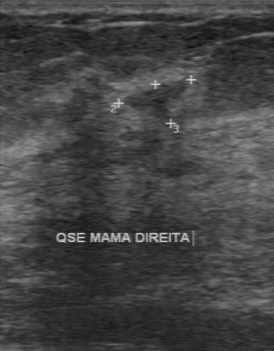
\includegraphics[height=2.75cm]{figures/busbra_benign.png} &
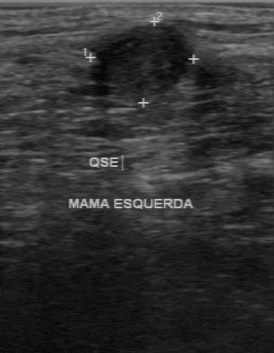
\includegraphics[height=2.75cm]{figures/busbra_malignant.png} &
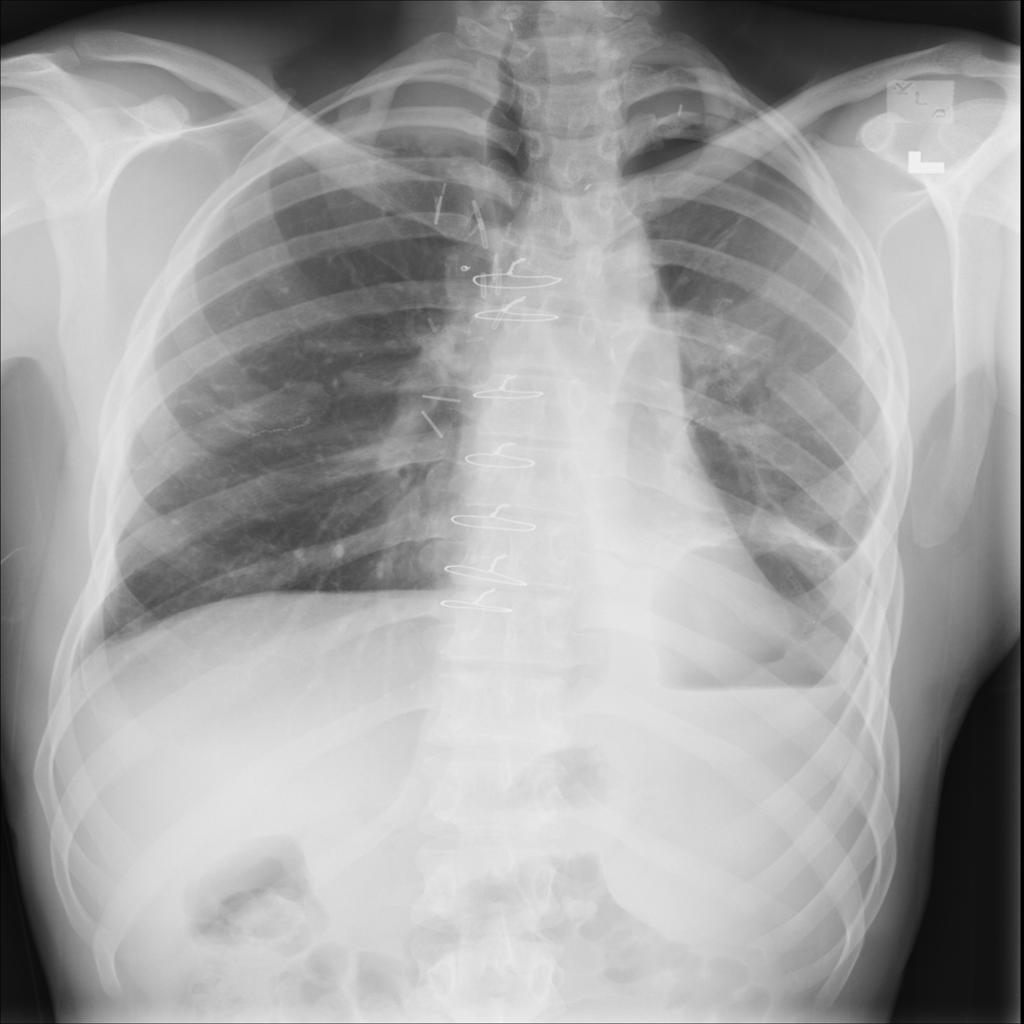
\includegraphics[height=2.75cm]{figures/bnvqa_chestxray_00001170_046.jpg} \\
\scriptsize (a) BUS-BRA, benign & \scriptsize (b) BUS-BRA, malignant & \scriptsize (c) BanglaMedVQA \\
\end{tabular}
\captionof{figure}{Example images from our samples. (a, b) BUS-BRA~\cite{gomezflores2024busbra} images bus\_0007-l and bus\_0001-l (CC~BY~4.0); only \medgemma{} classified both correctly. (c) ChestX-ray8~\cite{wang2017chestxray8} image 00001170\_046 with the question \bn{কোনও অস্বাভাবিকতা আছে কি?} (``Are any abnormalities present?''; reference \bn{হ্যাঁ}, ``yes''). RadImageNet-VQA images are not shown because its research-use agreement does not allow any part of the dataset to be reproduced.}
\label{fig_samples}
\end{minipage}
\par\medskip

\textbf{BUS-BRA}~\cite{gomezflores2024busbra} contains 1,875 breast ultrasound images from 1,064 patients with biopsy-proven benign or malignant labels (1,268 benign, 607 malignant). We chose it because the task is a clinically meaningful binary decision with a clear chance level, the labels are biopsy-proven, the dataset is openly licensed (CC~BY~4.0), and case identifiers let us take one image per case. We sampled 400 images from 400 different cases, excluding 20 cases used in an earlier pilot run and 13 cases flagged during data checks. The final ID list was frozen and verified with a SHA-256 hash before each run.

\textbf{RadImageNet-VQA}~\cite{butsanets2025radimagenetvqa} is built from the CT and MRI part of RadImageNet~\cite{mei2022radimagenet}. Its benchmark split has 9,000 questions on 1,000 images from eight anatomical regions. We kept the 7,000 yes/no and multiple-choice questions, so that every answer could be scored exactly, and grouped them by format and topic into five groups (Table~\ref{tab_prompts}): anatomy and pathology multiple choice, and anatomy, abnormality and pathology yes/no. We drew 100 questions per group.

\textbf{BanglaMedVQA}~\cite{ahmed2026banglamedvqa} has 7,000 Bangla questions, half on chest X-rays from ChestX-ray8~\cite{wang2017chestxray8} and half on figures from biomedical papers collected in MedICaT~\cite{subramanian2020medicat}. The questions fall into five categories: \emph{modality}, \emph{organ}, \emph{abnormality} (yes/no), \emph{condition} and \emph{position}. The question--answer pairs were generated from image metadata with Gemini and translated into Bangla; two medical specialists accepted 97.2\% and 97.6\% of a 1,000-pair subset~\cite{ahmed2026banglamedvqa}. We drew 50 questions for each source--category cell from the training splits (3,500 questions per source), at most one per image within a cell. The original paper reports results on the test splits (200 questions per source), so our numbers are not directly comparable with theirs. No model in our study was trained on BanglaMedVQA.

\subsection{Prompts and question types}
Each task used one fixed prompt for all models (Table~\ref{tab_prompts}), which was not changed once evaluation started. For BanglaMedVQA we used the dataset authors' published zero-shot system prompt verbatim and passed the Bangla question as the user message, to stay as close as possible to the original benchmark. Table~\ref{tab_prompts} also gives one real question from our samples for each of the ten question types. The RadImageNet-VQA groups separate \emph{where} the image is from (anatomy) from \emph{what is wrong} (abnormality, pathology); BanglaMedVQA makes a similar split between \emph{general} (modality, organ) and \emph{specialised} (abnormality, condition, position) categories~\cite{ahmed2026banglamedvqa}.

\begin{table*}[tb]
\centering
\caption{Top: the prompts (verbatim; line breaks shown as $\hookleftarrow$). The image is placed before the text in one user turn. Bottom: one example question from our samples for each question type. RadImageNet-VQA options are not reproduced (our result files store only the question text). English glosses for BanglaMedVQA are the dataset's own English versions; the models saw only the Bangla.}
\label{tab_prompts}
\footnotesize
\begin{tabular}{@{}p{2.7cm}p{14.3cm}@{}}
\toprule
\multicolumn{2}{@{}l}{\textbf{Prompts}} \\
BUS-BRA & \texttt{You are a medical assistant. Examine this breast ultrasound image.$\hookleftarrow$ Classify the lesion as exactly ONE of the following:$\hookleftarrow$ - benign: non-cancerous lesion$\hookleftarrow$ - malignant: cancerous lesion$\hookleftarrow\hookleftarrow$ Respond with ONLY the label: benign or malignant.} \\
RadImageNet-VQA, MCQ & \texttt{You are a medical assistant. Look at this image and answer the following multiple-choice question with ONLY the letter of the correct option (e.g. 'B'), nothing else.$\hookleftarrow\hookleftarrow$ Question: \{question\}$\hookleftarrow$ Options:$\hookleftarrow$ A. \{A\}$\hookleftarrow$ B. \{B\}$\hookleftarrow$ C. \{C\}$\hookleftarrow$ D. \{D\}} \\
RadImageNet-VQA, yes/no & \texttt{You are a medical assistant. Look at this image and answer the following question with ONLY the single word 'Yes' or 'No'.$\hookleftarrow\hookleftarrow$ Question: \{question\}} \\
BanglaMedVQA \newline (system prompt of~\cite{ahmed2026banglamedvqa}; user turn = Bangla question) & \texttt{You are a careful, clinically grounded medical vision-language assistant. Task: You will be given a medical image and a single question about that image (e.g., modality, organ, abnormality, condition, or the position of the condition). Your job is to look at the image and provide the exact, minimal answer to the question. CRITICAL: You must respond with ONLY the exact answer. No explanations, no sentences, no extra words. STRICT OUTPUT RULES: - ONE word or short phrase only - NO sentences or explanations - NO "This is..." or "The image shows..." - NO punctuation unless part of the answer} \\
\midrule
\end{tabular}
\begin{tabular}{@{}p{2.7cm}p{9.0cm}p{4.3cm}c@{}}
\multicolumn{2}{@{}l}{\textbf{Example questions}} & \textbf{Reference answer} & \textbf{Chance} \\
\multicolumn{4}{@{}l}{\textit{RadImageNet-VQA (CT/MRI), 100 questions per group}} \\
Anatomy, MCQ & Which of the following anatomical regions is depicted in this scan? & one letter (A--D) & 25\% \\
Anatomy, yes/no & Is the knee visible in the image? & yes & 50\% \\
Abnormality, yes/no & Does the lung look abnormal? & no & 50\% \\
Pathology, yes/no & Is the abdomen affected by bowel mass? & yes & 50\% \\
Pathology, MCQ & What is the most likely pathology in this image? & one letter (A--D) & 25\% \\
\multicolumn{4}{@{}l}{\textit{BanglaMedVQA (Bangla), 50 questions per category and source}} \\
Modality & \bn{এই গবেষণায় কোন ইমেজিং পদ্ধতি ব্যবহার করা হয়েছে?} (What imaging modality is used in this study?) & \bn{এক্স-রে} (X-ray) & -- \\
Organ & \bn{ছবিতে কোন অঙ্গটি দেখানো হয়েছে?} (What organ is depicted in the image?) & \bn{মস্তিষ্ক} (brain) & -- \\
Abnormality & \bn{কোনও অস্বাভাবিকতা আছে কি?} (Are any abnormalities present?) & \bn{হ্যাঁ} (yes) & 50\% \\
Condition & \bn{ছবিতে কী কী অবস্থা দেখা যাচ্ছে?} (What conditions are observed in the image?) & \bn{দুটি পাথর, এন্ডোক্লিপ} (two stones, endoclip) & -- \\
Position & \bn{নডিউলটি কোথায় অবস্থিত?} (Where is the nodule located?) & \bn{ডানদিকের মাঝখানে} (middle right) & -- \\
\bottomrule
\end{tabular}
\end{table*}

\subsection{Inference and answer parsing}
\label{sec_inference}
All models ran in bfloat16 with greedy decoding (no sampling), batch size~1 and seed~42, using each model's own chat template. Greedy decoding makes outputs deterministic for a given setup, and batch size~1 avoids padding effects. The output limit was 32 new tokens for BUS-BRA, 16 for RadImageNet-VQA and 96 for BanglaMedVQA (256 for \medvlm{}, so that a reasoning block, if produced, would not cut off the answer). The BUS-BRA runs pinned model revisions and library versions and ran on Kaggle T4 GPUs. In the two VQA runs, \medvlm{}'s own processor did not load with the installed \texttt{transformers} version, so we used the processor of its base model, \qwen{}-2B-Instruct; for BanglaMedVQA the Qwen processors were limited to $256$--$1280$ visual patches of $28\times28$ pixels.

Answers that could not be parsed would count as wrong, but every output was parseable. BUS-BRA answers had to be exactly \texttt{benign} or \texttt{malignant}; RadImageNet-VQA took the first standalone letter A--D or the first ``yes''/``no''; BanglaMedVQA answers were only stripped of whitespace, quotes and a final full stop or Bangla \emph{dari}. All 3,600 classification and closed-VQA outputs were a single word or letter, and no model produced \texttt{<think>} or \texttt{<answer>} tags in any task.

\subsection{Metrics and statistics}
For BUS-BRA and RadImageNet-VQA we report accuracy with 95\% Wilson intervals~\cite{wilson1927} and a one-sided exact binomial test against chance. For BUS-BRA we add sensitivity and specificity, and for yes/no questions the share of ``yes'' answers, since a balanced set makes any answer preference visible.

For BanglaMedVQA we follow the original paper and report exact match (EM), BERTScore F1~\cite{zhang2020bertscore} (cased multilingual BERT-base, layer~9, no rescaling) and LAVE~\cite{manas2024lave}, in which an LLM judge rates each answer between 0 and 1 against the reference. As in the original paper, the judge was GPT-4.1-mini with the paper's judge prompt, which shows only the reference and the answer, not the question; we used one call per answer at temperature~0, and no call failed. LAVE is our main Bangla metric because EM is close to zero for all models. We also checked LAVE with two rule-based audits that use no judge: whether a yes/no answer is correct in either language, and whether the modality named in a modality answer is correct.

Each medical model is compared with its general-purpose counterpart on the same items. We report the paired difference with a 95\% bootstrap interval (5,000 resamples of items), and for accuracy the exact McNemar test~\cite{mcnemar1947}.

%% ===========================================================================
\section{RESULTS AND ANALYSIS}
\label{sec_results}

\subsection{Main result: medical versus general-purpose model}
\label{sec_res_main}
Table~\ref{tab_pairs} compares each medical model with its general-purpose counterpart on all three tasks. The medical models did not show a consistent advantage under our shared direct-answer protocol.

\begin{table}[tb]
\centering
\caption{Medical model minus its general-purpose counterpart on the same items: difference in accuracy (BUS-BRA, RadImageNet-VQA) or LAVE (BanglaMedVQA), in percentage points, with 95\% paired bootstrap interval; exact McNemar $p$; share of identical answers.}
\label{tab_pairs}
\footnotesize
\setlength{\tabcolsep}{2.5pt}
\resizebox{\columnwidth}{!}{%
\begin{tabular}{@{}lcc@{}}
\toprule
 & \textbf{\medvlm{} $-$ \qwen{}} & \textbf{\medgemma{} $-$ \gemma{}} \\
\midrule
\textbf{BUS-BRA} & $0.0$ & $+7.3$ ($-0.3$, $15.0$) \\
 & \scriptsize identical answers on all 400 & \scriptsize $p=0.08$; 35\% identical \\
\addlinespace
\textbf{RadImageNet-VQA} & $+0.8$ ($-1.2$, $2.8$) & $-1.8$ ($-7.2$, $3.6$) \\
 & \scriptsize $p=0.57$; 93\% identical & \scriptsize $p=0.56$; 55\% identical \\
\addlinespace
\textbf{BanglaMedVQA} & $+0.8$ ($-0.3$, $2.0$) & $\mathbf{+7.4}$ ($4.8$, $10.0$) \\
 & \scriptsize 72\% identical & \scriptsize 36\% identical \\
\bottomrule
\end{tabular}}
\end{table}

\textbf{\medvlm{} behaved like a copy of \qwen{}.} It gave identical answers on every BUS-BRA image, on 93\% of RadImageNet-VQA questions and on 72\% of BanglaMedVQA questions, and none of the differences is distinguishable from zero. This fits its training: it was tuned on 600 MRI multiple-choice questions to write a reasoning block before a letter answer. Our prompts asked for a bare answer, the model complied, and the reinforcement learning left its direct answers essentially unchanged.

\textbf{\medgemma{} gave different answers, without a consistent score advantage.} Only 35--55\% of its answers matched \gemma{}'s. It obtained a higher Bangla judge score, higher but not significantly different accuracy on BUS-BRA, and lower but not significantly different accuracy on RadImageNet-VQA. The Bangla audit limits interpretation of that judge-score gain. The next three subsections show what each task adds to this picture.

\subsection{BUS-BRA: accuracy hides constant answers}
\label{sec_res_busbra}
Three of the four models scored at or near chance on BUS-BRA (Table~\ref{tab_busbra}), and the reason is visible in their answers: \qwen{} and \medvlm{} answered ``benign'' for all 400 images, and \gemma{} answered ``malignant'' for 391. On a balanced sample a constant answer earns exactly 50\%. \gemma{}'s 98\% sensitivity was accompanied by only 2.5\% specificity: it labelled almost every image malignant.

\medgemma{} was the only model with accuracy significantly above chance. It reached 57.5\% (95\% CI 52.6--62.3\%; $p=0.0016$, still significant after Bonferroni correction for four models). It leaned towards ``benign'', however, and misclassified 118 of the 200 malignant images. Its gain over \gemma{} (+29 images) was not significant in the paired test (144 images correct only for \medgemma{} against 115 only for \gemma{}). Thus, above-chance accuracy does not establish superiority over \gemma{} or isolate dependence on image content.

\begin{table}[tb]
\centering
\caption{BUS-BRA results (400 images, 200 per class). ``Malig.'' = number of ``malignant'' answers; Sens./Spec.\ = sensitivity/specificity for malignant (\%); $p$: one-sided binomial test against 50\%.}
\label{tab_busbra}
\footnotesize
\setlength{\tabcolsep}{2.5pt}
\resizebox{\columnwidth}{!}{%
\begin{tabular}{@{}lccccc@{}}
\toprule
\textbf{Model} & \textbf{Acc.\ \% (95\% CI)} & \textbf{Malig.} & \textbf{Sens.} & \textbf{Spec.} & $p$ \\
\midrule
\qwen{}-2B & 50.0 (45.1--54.9) & 0 & 0.0 & 100.0 & 0.52 \\
\medvlm{} & 50.0 (45.1--54.9) & 0 & 0.0 & 100.0 & 0.52 \\
\gemma{}~4B & 50.3 (45.4--55.1) & 391 & 98.0 & 2.5 & 0.48 \\
\medgemma{}~4B & \textbf{57.5} (52.6--62.3) & 134 & 41.0 & 74.0 & 0.002 \\
\bottomrule
\end{tabular}}
\end{table}

\subsection{RadImageNet-VQA: anatomy is easy, disease is not}
\label{sec_res_radimagenet}
Overall accuracy was similar for all four models: 64.2\% (\qwen{}), 65.0\% (\medvlm{}), 63.0\% (\gemma{}) and 61.2\% (\medgemma{}), against a chance level of 40\%. The question groups tell a clearer story (Fig.~\ref{fig_radimagenet}). Every model recognised anatomy well (79--88\% on both anatomy groups), but disease scores were substantially lower: 52--61\% on abnormality and pathology yes/no (chance 50\%) and 32--37\% on pathology multiple choice (chance 25\%). With 100 questions per group the 95\% interval is about $\pm$9 points, so several of the disease scores cannot be separated from guessing. A large anatomy--disease gap remained for both medical models; \medgemma{} was below \gemma{} on both anatomy groups, although neither difference is significant ($p=0.39$ and $0.79$).

\begin{figure}[tb]
\centering
\begin{tikzpicture}
\begin{axis}[modelbars, ymax=100, ylabel={Accuracy (\%)},
  symbolic x coords={AM,AY,BY,PY,PM},
  xticklabels={Anatomy\\MCQ, Anatomy\\yes/no, Abnorm.\\yes/no, Pathology\\yes/no, Pathology\\MCQ}]
\addplot[fill=cQwen, draw=black] coordinates {(AM,87) (AY,88) (BY,55) (PY,57) (PM,34)};
\addplot[fill=cMedVLM, draw=black] coordinates {(AM,88) (AY,86) (BY,61) (PY,57) (PM,33)};
\addplot[fill=cGemma, draw=black] coordinates {(AM,84) (AY,81) (BY,52) (PY,61) (PM,37)};
\addplot[fill=cMedGemma, draw=black] coordinates {(AM,80) (AY,79) (BY,55) (PY,60) (PM,32)};
\legend{Qwen2-VL, MedVLM-R1, Gemma 3, MedGemma}
\draw[dashed, gray] ([xshift=-14pt]axis cs:AM,25) -- ([xshift=14pt]axis cs:AM,25);
\draw[dashed, gray] ([xshift=-14pt]axis cs:AY,50) -- ([xshift=14pt]axis cs:AY,50);
\draw[dashed, gray] ([xshift=-14pt]axis cs:BY,50) -- ([xshift=14pt]axis cs:BY,50);
\draw[dashed, gray] ([xshift=-14pt]axis cs:PY,50) -- ([xshift=14pt]axis cs:PY,50);
\draw[dashed, gray] ([xshift=-14pt]axis cs:PM,25) -- ([xshift=14pt]axis cs:PM,25);
\end{axis}
\end{tikzpicture}
\caption{RadImageNet-VQA accuracy by question group (100 questions each). Dashed lines mark chance. Light bars are general models, dark bars their medical versions.}
\label{fig_radimagenet}
\end{figure}

\textbf{When the image does not decide, the models fall back on preferences} (Table~\ref{tab_prefs}). Because each yes/no group was balanced, an unbiased model would say ``yes'' about half the time. \gemma{} said ``yes'' to 74\% of yes/no questions, including 98 of the 100 abnormality questions. \medgemma{}, trained from it, leaned the other way, with 42\% ``yes'' overall and 32\% on pathology. Medical training did not remove the bias; it reversed it, and on abnormality questions both models ended up near chance from opposite directions. On pathology multiple choice the correct letters were spread evenly (A~25, B~22, C~25, D~28), yet each pair favoured one letter: B for the Gemma pair, C for the Qwen pair. This matches the option-letter bias known for language models~\cite{zheng2024mcqbias} and suggests the preference is inherited from the base model.

\begin{table}[tb]
\centering
\caption{RadImageNet-VQA answer preferences. Share of ``yes'' answers per yes/no group (true share 50\%), and the most chosen letter on pathology MCQ with its count (the correct letter was B in 22 of 100 questions, C in 25).}
\label{tab_prefs}
\footnotesize
\setlength{\tabcolsep}{3pt}
\resizebox{\columnwidth}{!}{%
\begin{tabular}{@{}lcccc@{}}
\toprule
 & \textbf{Qwen2} & \textbf{MedVLM} & \textbf{Gemma3} & \textbf{MedGemma} \\
\midrule
``Yes'', anatomy (\%) & 42 & 42 & 49 & 55 \\
``Yes'', abnormality (\%) & 77 & 69 & 98 & 39 \\
``Yes'', pathology (\%) & 43 & 47 & 75 & 32 \\
``Yes'', all yes/no (\%) & 54 & 53 & 74 & 42 \\
\midrule
Top letter, path.\ MCQ & C (37) & C (35) & B (35) & B (42) \\
\bottomrule
\end{tabular}}
\end{table}

The four models also failed together: all of them were wrong on the same 65 questions (13\%). Accuracy varied by body region (hip was hardest for every model, 37--53\% on 38 questions), but most region-level cells are too small to interpret.

\subsection{BanglaMedVQA: a judge-score gain that needs care}
\label{sec_res_bangla}
BanglaMedVQA is the only task with a statistically detected aggregate score gain for a medical model (Table~\ref{tab_bangla}): \medgemma{} reached 31.5\% LAVE against 24.1\% for \gemma{}. This is a judge-score gain whose interpretation depends on the audit below. The two Qwen-family models were close to each other at about 15--16\%. Exact match was near zero for all models, which is why LAVE carries the comparison.

\begin{table}[tb]
\centering
\caption{BanglaMedVQA results (500 questions). EM = exact match (\%). LAVE with 95\% bootstrap interval. ``No Bangla'' = share of answers containing no Bangla script (\%).}
\label{tab_bangla}
\footnotesize
\setlength{\tabcolsep}{3pt}
\resizebox{\columnwidth}{!}{%
\begin{tabular}{@{}lcccc@{}}
\toprule
\textbf{Model} & \textbf{EM} & \textbf{BERTScore} & \textbf{LAVE (95\% CI)} & \textbf{No Bangla} \\
\midrule
\qwen{}-2B & 0.0 & 68.6 & 15.1 (12.5--17.8) & 82.0 \\
\medvlm{} & 0.0 & 68.4 & 16.0 (13.4--18.7) & 89.2 \\
\gemma{}~4B & 2.4 & 69.0 & 24.1 (20.9--27.3) & 90.0 \\
\medgemma{}~4B & 1.6 & \textbf{71.4} & \textbf{31.5} (28.1--34.9) & 98.2 \\
\bottomrule
\end{tabular}}
\end{table}

\textbf{The judge-score gain is in the easy categories.} Fig.~\ref{fig_bangla} shows the same anatomy-versus-disease pattern as RadImageNet-VQA. Modality was the easiest category for every model, and organ questions were answered well only by the Gemma pair. Condition, abnormality and position stayed between 0\% and 13\% LAVE for all four models in both sources. \medgemma{}'s lead over \gemma{} came almost entirely from chest X-ray organ (+30.6 points) and chest X-ray modality (+20.4) questions, the only two cells whose paired intervals exclude zero. Modality is also close to a base-rate question here: X-ray is the reference for 56 of our 100 modality questions.

\begin{figure}[tb]
\centering
\begin{tikzpicture}
\begin{axis}[modelbars, ymax=80, ylabel={LAVE (\%)},
  symbolic x coords={Mo,Or,Co,Ab,Po},
  xticklabels={Modality, Organ, Condition, Abnormality, Position}]
\addplot[fill=cQwen, draw=black] coordinates {(Mo,55.8) (Or,3.3) (Co,8.3) (Ab,6.1) (Po,2.2)};
\addplot[fill=cMedVLM, draw=black] coordinates {(Mo,56.5) (Or,5.3) (Co,8.0) (Ab,6.4) (Po,3.7)};
\addplot[fill=cGemma, draw=black] coordinates {(Mo,60.7) (Or,47.1) (Co,6.6) (Ab,0.0) (Po,6.1)};
\addplot[fill=cMedGemma, draw=black] coordinates {(Mo,73.3) (Or,63.1) (Co,11.1) (Ab,5.0) (Po,4.9)};
\legend{Qwen2-VL, MedVLM-R1, Gemma 3, MedGemma}
\end{axis}
\end{tikzpicture}
\caption{BanglaMedVQA LAVE by question category, averaged over the chest X-ray and MedICaT sources (100 questions per category).}
\label{fig_bangla}
\end{figure}

\textbf{The models mostly answered in English.} Although every question was in Bangla, 82--98\% of each model's answers contained no Bangla script; \medgemma{}, the best model, answered in Bangla least often. When the Qwen models did answer in Bangla the answer was often meaningless; their most frequent answer to chest X-ray organ questions was \bn{লাইন} (``line''). They also answered some MedICaT questions with a bare option letter although no options were given (39 answers for \qwen{}, 27 for \medvlm{}). Several models repeated one stock answer: \medvlm{} said ``pneumonia'' to 37 of the 50 chest X-ray condition questions. On the balanced abnormality questions, the yes/no preferences from RadImageNet-VQA appeared again: the Qwen models never answered ``yes'', while 62 of \medgemma{}'s 79 clear yes/no answers were ``yes''.

\textbf{The metric under-credits correct English answers} (Table~\ref{tab_audit}). The LAVE judge sees only the Bangla reference and the model's answer. After normalising reference punctuation, \medgemma{} answered 36 Bangla ``yes'' questions with the English ``Yes''; every one of these correct answers scored 0. Across all abnormality questions, its 53 correct English yes/no answers scored 0, while its five correct Bangla yes/no answers scored 1.0. Some of the Qwen models' correct ``no'' answers received credit, but none of \gemma{}'s 12 correct yes/no answers did. Correct ``CT'' answers to modality questions averaged about 0.31 LAVE against about 0.87 for correct ``X-ray'' answers, for every model. Answers assigned zero LAVE still averaged about 66--70 BERTScore without rescaling, and the metrics' rank correlation was only 0.27--0.43; this disagreement does not independently establish correctness.

\begin{table}[tb]
\centering
\caption{Audit of LAVE using rule-based checks (100 questions per category). Top: correct English/Bangla yes/no answers, including explicit negative phrases, after case and punctuation normalisation; counts credited by LAVE ($>0$). Bottom: broad modality matches using English/Bangla synonyms, including radiography as X-ray and fMRI as MRI.}
\label{tab_audit}
\footnotesize
\setlength{\tabcolsep}{3pt}
\resizebox{\columnwidth}{!}{%
\begin{tabular}{@{}lcccc@{}}
\toprule
 & \textbf{Qwen2} & \textbf{MedVLM} & \textbf{Gemma3} & \textbf{MedGemma} \\
\midrule
Correct yes/no answers & 31 & 34 & 12 & 58 \\
\quad credited by LAVE & 8 & 11 & 0 & 5 \\
\midrule
Correct modality (rule) & 82 & 84 & 99 & 99 \\
Modality LAVE (\%) & 55.8 & 56.5 & 60.7 & 73.3 \\
\bottomrule
\end{tabular}}
\end{table}

These examples show under-crediting of correct answers, but do not establish a lower bound on correctness or quantify how much of the overall model gap is due to answer language. This limits interpretation of the LAVE scores in Table~\ref{tab_bangla}. The original paper reported 19.85\% zero-shot LAVE for \medgemma{}~4B on the test split~\cite{ahmed2026banglamedvqa}, against our 31.5\% on a different sample; the scores are not directly comparable. Table~\ref{tab_examples} shows example answers.

\begin{table*}[tb]
\centering
\caption{Example BanglaMedVQA answers from our sample, with each answer's LAVE score in brackets. English glosses are for the reader. The second row is the same kind of question as the first, answered correctly in English by \medgemma{} and scored 0.}
\label{tab_examples}
\footnotesize
\setlength{\tabcolsep}{3pt}
\begin{tabular}{@{}p{1.9cm}p{3.6cm}p{2.3cm}p{2.1cm}p{2.1cm}p{2.3cm}p{2.1cm}@{}}
\toprule
\textbf{Source / type} & \textbf{Question} & \textbf{Reference} & \textbf{\qwen{}} & \textbf{\medvlm{}} & \textbf{\gemma{}} & \textbf{\medgemma{}} \\
\midrule
Chest X-ray, abnormality & \bn{কোনও অস্বাভাবিকতা আছে কি?} (Any abnormality?) & \bn{হ্যাঁ} (yes) & no [0.0] & no [0.0] & Consolidation [0.0] & \bn{হ্যাঁ} [1.0] \\
MedICaT, \newline abnormality & \bn{ছবিতে কি কোনো অস্বাভাবিকতা দেখা যাচ্ছে?} (Is an abnormality visible?) & \bn{হ্যাঁ} (yes) & A: A mass in the right temporal lobe [0.0] & A: There is no abnormality [0.0] & Lesions [0.0] & Yes [0.0] \\
MedICaT, organ & \bn{ছবিতে কোন অঙ্গটি দেখানো হয়েছে?} (Which organ?) & \bn{মস্তিষ্ক} (brain) & A [0.0] & A [0.0] & \bn{মস্তিষ্কের} [0.8] & \bn{মস্তিষ্ক} [1.0] \\
Chest X-ray, position & \bn{নডিউলটি কোথায় অবস্থিত?} (Where is the nodule?) & \bn{ডানদিকের মাঝখানে} (middle right) & lung [0.0] & lung [0.0] & \bn{ডান ফুসফুস} (right lung) [0.3] & Lung [0.0] \\
MedICaT, \newline position & (Where is the diffusely hyperechoic myocardium with acoustic shadowing?) & \bn{বাম ভেন্ট্রিকল} (left ventricle) & C [0.0] & A [0.0] & Left ventricle [0.9] & Heart [0.0] \\
\bottomrule
\end{tabular}
\end{table*}

\subsection{Discussion}
Across the three tasks the four models behaved similarly. They recognised \emph{what kind of image} they were given (modality, anatomy) much better than \emph{what was wrong} in it. When the image did not settle the answer, they used a fixed preference (one class label, ``yes'' or ``no'', one option letter, one stock disease name), and this preference was either kept or simply reversed by medical training. In Bangla they mostly answered in English, which the standard metrics do not score fairly.

Each task contributes a different piece of evidence to the main finding. BUS-BRA shows that the reinforcement-learning adaptation did not change behaviour at all, and that \medgemma{}'s improvement over a chance-level base is weak and not significant. RadImageNet-VQA shows that neither adaptation closed the gap between anatomy and disease, even though \medvlm{} was trained on MRI questions of a similar style. BanglaMedVQA gives the only clear gain, but it comes from general questions, and its size depends on how answers in the wrong language are scored.

Two practical points follow. First, balanced samples and answer distributions were essential: on BUS-BRA's natural class mix (68\% benign) the always-``benign'' Qwen models would have reached about 68\% accuracy, and on the full RadImageNet-VQA benchmark, where 72\% of abnormality questions have the answer ``yes'', \gemma{}'s ``yes'' preference would look like skill. Reporting the share of each answer costs nothing and exposed every such case. Second, a medical model should be compared with its own base model before claiming an improvement, as Jeong et al.~\cite{jeong2024medadapt} also argue. For the small models we tested, general medical training was not enough to improve zero-shot diagnosis; this points to the need for training methods and high-quality data aimed specifically at diagnostic questions and at low-resource languages.

%% ===========================================================================
\section{LIMITATIONS}
\label{sec_limitations}

\textbf{One shared prompt per task.} An identical prompt isolates the effect of the weights, but does not give each model its best conditions. \medvlm{} was trained to reason in \texttt{<think>} tags before answering (its model card generates up to 1,024 tokens); we tested it only in direct-answer mode, so we cannot say whether its reasoning mode helps. \medgemma{} might also do better with its own recommended prompts.

\textbf{Small samples and one run.} Each RadImageNet-VQA group has 100 questions and each BanglaMedVQA cell 50, so group-level intervals are wide. Each item was run once with greedy decoding.

\textbf{Text outputs only, no image-ablation control.} We stored decoded answers, not probabilities, so we cannot compute AUC on BUS-BRA; a model with a strong label preference might still rank lesions well. We also did not run blank-image controls, which would show how much each answer depends on the image.

\textbf{Bangla evaluation.} LAVE relies on a proprietary judge that sees no question and scored correct English answers inconsistently, and BERTScore was computed without rescaling. The BanglaMedVQA references were LLM-generated and machine-translated, with expert checks on a subset only. We did not run the English versions of the questions, which would separate visual errors from language errors, and our train-split sample differs from the original paper's test split.

\textbf{Possible training-data overlap.} \medvlm{}'s 600 MRI training pairs were drawn from the HuatuoGPT-Vision evaluation collection, which combines several benchmarks including OmniMedVQA~\cite{pan2025medvlmr1}. This does not establish overlap with our samples. Complete training provenance is unavailable for the evaluated models, so we cannot rule out prior exposure for either medical or general-purpose models, or determine its effect on their comparison.

\textbf{Reproducibility and scope.} Model revisions and library versions were pinned for BUS-BRA but not recorded for the two VQA tasks. We tested two pairs of 2B and 4B models on three datasets; larger models or fine-tuned use may behave differently. None of these results is a clinical evaluation.

%% ===========================================================================
\section{CONCLUSIONS}
\label{sec_conclusion}

We compared two small medical VLMs with the general-purpose models they were built from, under identical zero-shot conditions, on breast ultrasound classification, closed-ended CT/MRI question answering and open-ended Bangla question answering. Medical adaptation did not consistently improve performance: \medvlm{} was nearly indistinguishable from \qwen{}, and \medgemma{} improved on \gemma{} only in Bangla, mainly on modality and organ questions. All four models recognised anatomy far better than disease, fell back on fixed answer preferences, and mostly answered Bangla questions in English. Future work should compare medical models with their base models, report answer distributions alongside accuracy, test each model in its intended prompting mode, and develop training methods and data aimed at diagnostic reasoning and low-resource languages.

%% Double-blind: no acknowledgements in the review version.

\bibliographystyle{ijcvsplatex-num}
\bibliography{references}

\end{document}
